\documentclass[12pt]{article}
\usepackage[utf8]{inputenc}
\usepackage{amsmath}
\usepackage{amsfonts}
\usepackage{amssymb}
\usepackage{graphicx}
\usepackage{geometry}
\usepackage{xcolor}
\usepackage{listings}

\author{Ben Kallus}
\date{Sunday, May 16}
\title{Interfacing with a PS/2 Keyboard to Make Music}

\begin{document}
\maketitle

\section*{Reading from the Keyboard}

    I started this project by wiring up the keyboard and writing a Python program for the Feather to interface with the keyboard.
    However, the program didn't work at all; scan codes that I read were inconsistent and nonsensical.
    I believe this effect was caused by CircuitPython being too slow to speak PS/2.

    PS/2 is a specification for a keyboard and mouse connector and protocols for interfacing with those devices.\footnote{I also recently came into possession of a steering whee
l video game controller that uses the PS/2 connector. I'm assuming it speaks the mouse protocol, but I haven't checked yet.}
    PS/2 gets its name from the IBM Personal System/2, a line of computers from the late 1980s.
    Despite its age, the PS/2 protocol remains popular among a subset of computer users for its low latency compared to USB.
    The PS/2 protocol makes use of 4 pins, although the connector features some extra unused pins.
    There are two pins for +5V and ground, one for clock, and one for data.
    The clock pulses once for each data bit.
    Pressing a key on a PS/2 keyboard sends a scan code over the data line.
    A scan code consists of a start bit, 8 data bits, a parity bit, and a stop bit.
    The start bit is always 0, and the stop bit is always 1.
    The parity bit is 0 if and only if the data bits have odd Hamming weight.
    The data bits are sent in decreasing order of bit significance.

    A PS/2 clock period takes 80 $\mu$s.
    A \texttt{for} loop that calls \texttt{time.monotonic\_ns} repeatedly and adds the results to an array will record the time about once every 40-48 $\mu$s.
    Thus, a Feather running CircuitPython could conceivably miss an entire half period of a PS/2 clock cycle, so I needed to use something faster.
    Unintuitively, I decided to switch to an Arduino Uno clocked at 16MHz, 3 times slower than the Feather.
    However, because I programmed the Uno in C, it was fast enough to read scan codes accurately.
    For some reason, the Uno reads from the data line three times per clock cycle, even though I intended for it to read once per clock cycle.
    I didn't fix this bug elegantly; I just threw out two out of every three bits read.
    I suppose this could be made into a feature by using the redundancy to correct errors.
    It's worth noting that I did not implement support for pressing multiple keys simultaneously, and there are a few unimplemented keys on the keyboard, such as the modifier keys, Pause|Break, Home/End, and Page Up/Page Down.
    I would have liked to support simultaneous key presses, but it would require catching scan codes faster than I can send them over the UART at 115200 baud.

\section*{Interfacing with a Computer}

    Once a scan code has been read, the next step is to send it to a computer over USB.
    The Uno has no official HID library, so I chose to send the scan code from the Uno to a Feather, which does have an HID library, although I had to install it myself.
    Initially, I planned on using IR instead of UART, but I hooked up my receiver backward and fried it.
    On the other end of the UART is a Feather running a Python program that collects the scan code, then looks up its corresponding key.
    The tables mapping scan codes to keys that I could find online did not perfectly match is keyboard's layout, so I had to construct about a third of the table myself.
    Using Adafruit's \texttt{adafruit\_hid} CircuitPython library, the Feather sends the appropriate keypress over USB to my laptop.
    Thus, I am able to type this sentence on a PS/2 keyboard on a computer with no native PS/2 interface.
    I think that's pretty cool.
    Once my keyboard was finally functioning as a keyboard, I decided to expand the scope of my project.

\section*{Making Music}

    I never use scroll lock, so on my keyboard, the scroll lock key has been repurposed; pressing scroll lock initiates music mode.
    In music mode, the Feather does not send keystrokes to the laptop.
    Instead, the Feather waits for the user to type the name of a note matching the following regular expression: \texttt{[A-Ga-g][BbSs]?[0-8]}, then plays that note over a speaker connected to the Feather through an LF356N op-amp.
    For example, typing ``Db4" or ``Cs4" will play a square wave at 277 Hz.
    Typing the names of notes in this way is a challenge, but it's still pretty fun to play.
    To exit music mode, just press the reset button on the Feather.
    I've emailed you a rendition of Frère Jacques played on this instrument, and would love to give you a demonstration if you're in the lab this week.
    You may notice that the pitches aren't perfectly in tune.
    This is because CircuitPython's \texttt{PWMOut} class accepts only integer frequencies, lower pitches are less accurate than higher ones.

\newpage\section*{Schematic}

    Shown below is a schematic for my project.
    Obvious power and ground wires are omitted for clarity.

    \begin{center}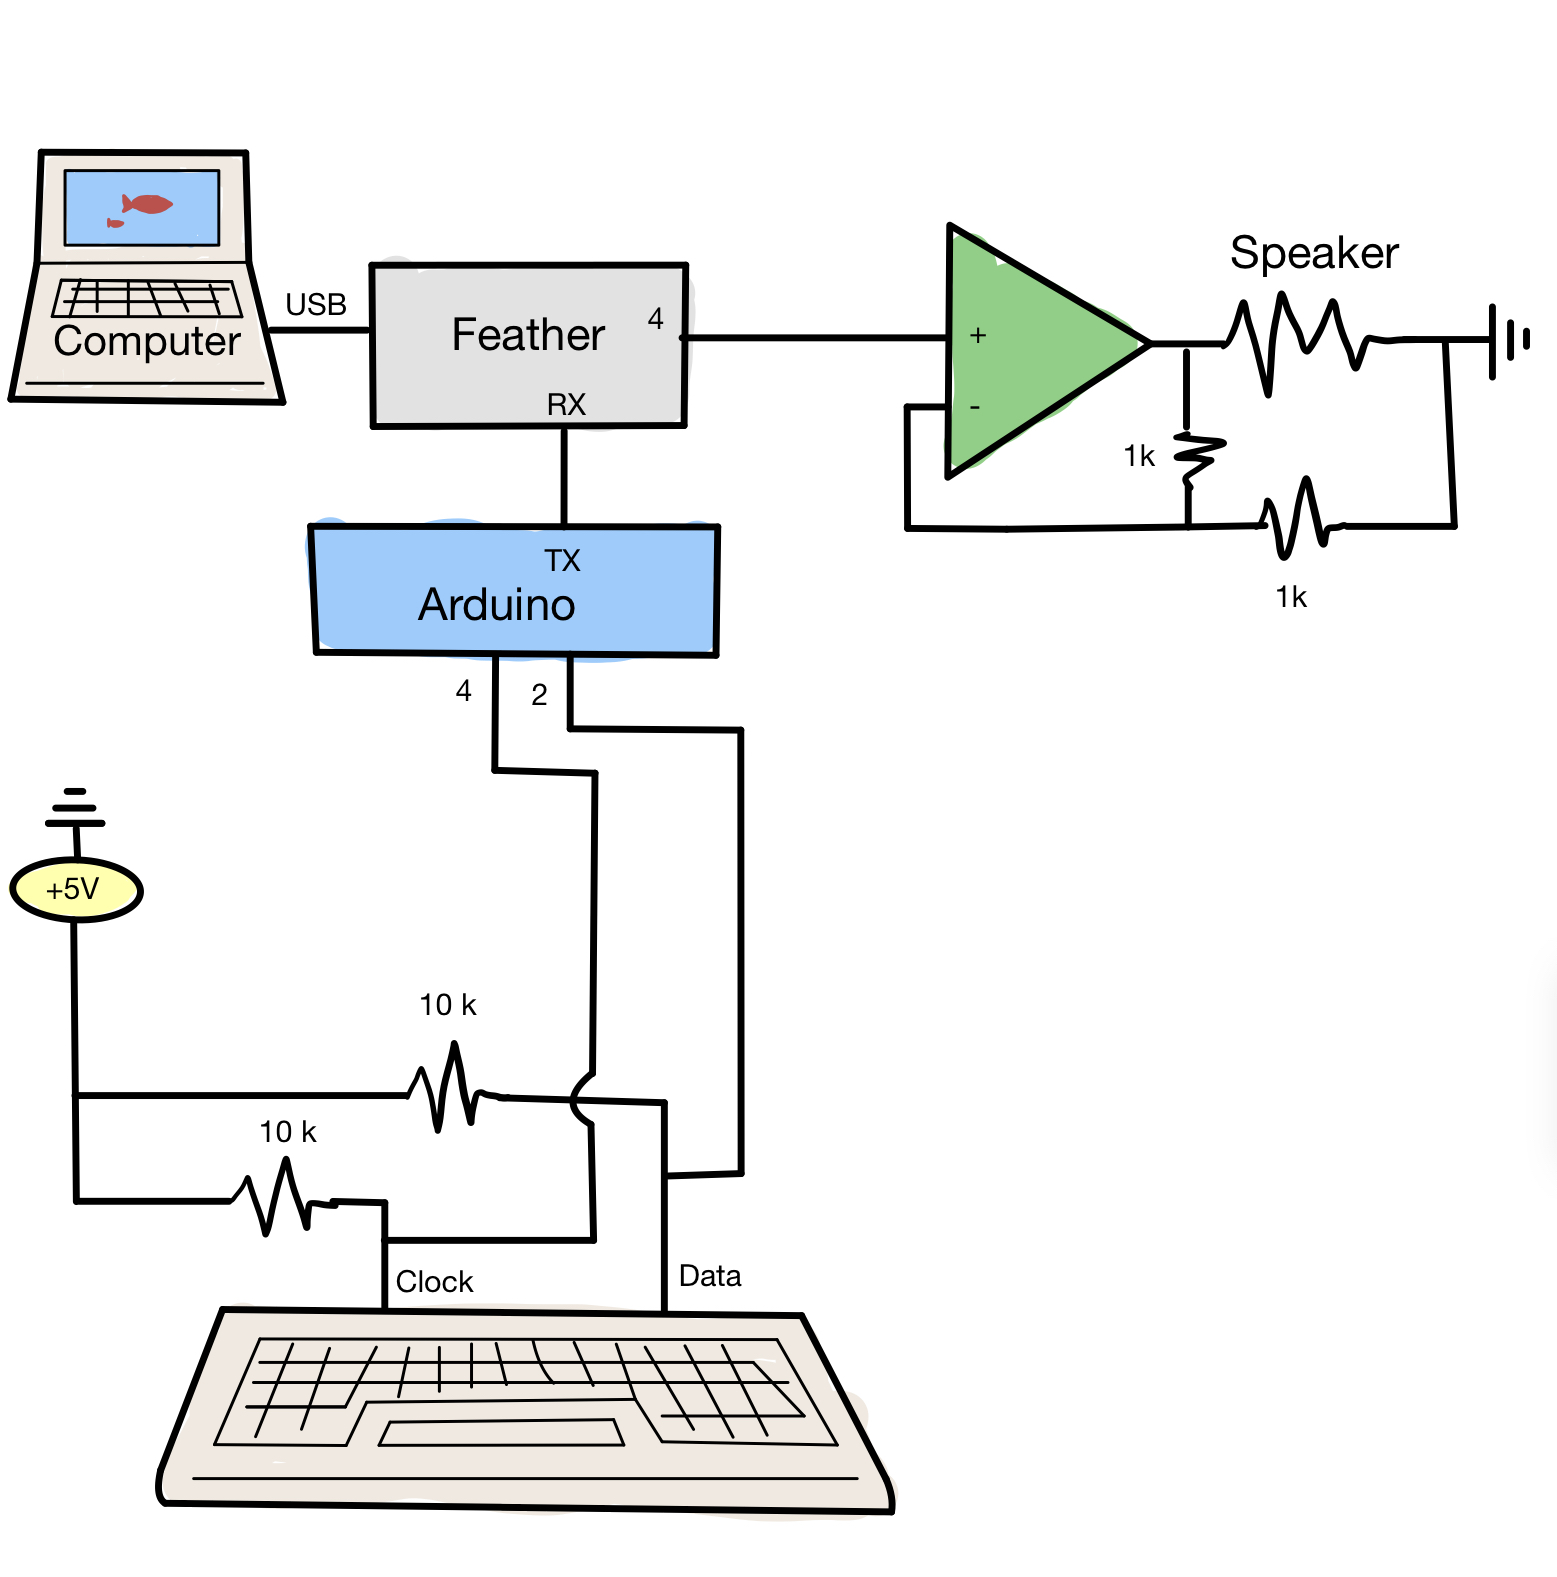
\includegraphics[scale=.2]{schematic.jpg}\end{center}

\section*{Code}

    Both my Python program and my C program are included along with this file in my final project submission on Blackboard.

\end{document}
